\documentclass[utf8]{ctexart}
\usepackage{graphicx}
\usepackage{amsmath, amssymb, amsthm}
\usepackage{geometry}
\usepackage{enumitem}
\usepackage{xcolor}
\usepackage{mdframed}
\usepackage{tikz}

\usetikzlibrary{arrows.meta,positioning,calc}
\usepackage{booktabs}
\usepackage{array}

\geometry{margin=2cm}

\definecolor{critical}{RGB}{200,40,40}
\definecolor{nodeblue}{RGB}{52,120,200}
\definecolor{nodegray}{RGB}{215,228,242}
\definecolor{critnodebg}{RGB}{255,218,218}

\usetikzlibrary{graphs, positioning, arrows.meta}

\geometry{a4paper, margin=2.5cm}

% 定理环境
\newtheoremstyle{mystyle}
  {8pt}{8pt}{\kaishu}{0pt}{\bfseries}{}{1em}{}
\theoremstyle{mystyle}
\newtheorem{theorem}{定理}
\newtheorem{lemma}{引理}

% 好看的题目框
\newmdenv[
  linecolor=black!40,
  linewidth=1pt,
  backgroundcolor=gray!8,
  roundcorner=5pt,
  innertopmargin=8pt,
  innerbottommargin=8pt,
]{problembox}

\title{\textbf{离散数学2\quad 作业8}}
\date{\today}
\author{李子嘉 2024012325}
\begin{document}
\maketitle

\section*{题目1}

\begin{problembox}
    已知连通图 $G$ 的基本关联矩阵是：
\[
\begin{bmatrix}-1 & 1 & 0 & 0 & 0 & 1 & 0 & 0 \\ 1 & 0 & 0 & 1 & 1 & 0 & 0 & 0 \\ 0 & -1 & -1 & 0 & 0 & 0 & -1 & 0 \\ 0 & 0 & 1 & -1 & 0 & 0 & 0 & -1\end{bmatrix}
\]
求：
\begin{enumerate}
    \item 以 ${e_3, e_4, e_6, e_7}$ 为树的基本回路矩阵
    \item 以 ${e_2, e_5, e_6, e_8}$ 为树的基本割集矩阵
\end{enumerate}
\end{problembox}
\textbf{解：} 
\subsection*{第一问}
我们按照课堂上的标准流程，先整理关联矩阵，将树边放到后面，余树边放到前面，并做拆分，得到两矩阵 $B_{11}$ 和 $B_{12}$：
\[
B_{11} = \begin{bmatrix}-1 & 1 & 0 & 0 \\ 1 & 0 & 1 & 0 \\ 0 & -1 & 0 & 0 \\ 0 & 0 & 0 & -1\end{bmatrix}
B_{12} = \begin{bmatrix}0 & 0 & 1 & 0 \\ 0 & 1 & 0 & 0 \\ -1 & 0 & 0 & -1 \\ 1 & -1 & 0 & 0\end{bmatrix}
\]
随后计算 $C_{f12} = -B_{11}^{T}B_{12}^{-T}$，与单位矩阵拼接得到基本回路矩阵 $C_f$：
\[
C_f = \begin{bmatrix}1 & 0 & 0 & 0 & -1 & -1 & 1 & 1 \\ 0 & 1 & 0 & 0 & 0 & 0 & -1 & -1 \\ 0 & 0 & 1 & 0 & -1 & -1 & 0 & 1 \\ 0 & 0 & 0 & 1 & 1 & 0 & 0 & -1\end{bmatrix}
\]
它的列分别对应边 $e_1, e_2, e_5, e_8, e_3, e_4, e_6, e_7$。
\subsection*{第二问}
同样地，我们先整理关联矩阵，将树边放到后面，余树边放到前面，并做拆分，得到两矩阵 $B_{11}$ 和 $B_{12}$：
\[
B_{11} = \begin{bmatrix}-1 & 0 & 0 & 0 \\ 1 & 0 & 1 & 0 \\ 0 & -1 & 0 & -1 \\ 0 & 1 & -1 & 0\end{bmatrix}
B_{12} = \begin{bmatrix}1 & 0 & 1 & 0 \\ 0 & 1 & 0 & 0 \\ -1 & 0 & 0 & 0 \\ 0 & 0 & 0 & -1\end{bmatrix}
\]
随后计算 $S_{f12} = -B_{11}^{T}B_{12}^{-T}$，与单位矩阵拼接得到基本割集矩阵 $S_f$：
\[
S_f = \begin{bmatrix}0 & 1 & 0 & 1 & 1 & 0 & 0 & 0 \\ 1 & 0 & 1 & 0 & 0 & 1 & 0 & 0 \\ -1 & -1 & 0 & -1 & 0 & 0 & 1 & 0 \\ 0 & -1 & 1 & 0 & 0 & 0 & 0 & 1\end{bmatrix}
\]
它的列分别对应边 $e_1, e_3, e_4, e_7, e_2, e_5, e_6, e_8$。

若按照题目要求的顺序，我们可以对矩阵进行列交换，得到最终结果：
\[
C_f = \begin{bmatrix}0 & 1 & 1 & 0 & 0 & 0 & 1 & 0 \\ 1 & 0 & 0 & 1 & 1 & 0 & 0 & 0 \\ -1 & 0 & -1 & 0 & 0 & 1 & -1 & 0 \\ 0 & 0 & -1 & 1 & 0 & 0 & 0 & 1\end{bmatrix}
\]
\newpage
\section*{题目2}
\begin{problembox}
10个树叶的权值分别为 $20, 7, 88, 100, 6, 13, 18, 30, 7, 16$，求其构造的哈夫曼树的带权路径总长。
\end{problembox}
\textbf{解：} 我们按照哈夫曼树的构造方法，首先将所有权值放入一个优先队列中，每次取出权值最小的两个节点合并成一个新节点，并将新节点的权值重新加入队列，直到队列中只剩下一个节点为止。每次合并时，我们记录下新节点的权值，并在最后计算带权路径总长。
具体步骤如下：
\begin{enumerate}
    \item 初始队列：$[6, 7, 7, 13, 16, 18, 20, 30, 88, 100]$
    \item 合并 $6$ 和 $7$，得到新节点权值 $13$，队列更新为 $[7, 13, 13, 16, 18, 20, 30, 88, 100]$
    \item 合并 $7$ 和 $13$，得到新节点权值 $20$，队列更新为 $[13, 16, 18, 20, 20, 30, 88, 100]$
    \item 合并 $13$ 和 $16$，得到新节点权值 $29$，队列更新为 $[18, 20, 20, 29, 30, 88, 100]$
    \item 合并 $18$ 和 $20$，得到新节点权值 $38$，队列更新为 $[20, 29, 30, 38, 88, 100]$
    \item 合并 $20$ 和 $29$，得到新节点权值 $49$，队列更新为 $[30, 38, 49, 88, 100]$
    \item 合并 $30$ 和 $38$，得到新节点权值 $68$，队列更新为 $[49, 68, 88, 100]$
    \item 合并 $49$ 和 $68$，得到新节点权值 $117$，队列更新为 $[88, 100, 117]$
    \item 合并 $88$ 和 $100$，得到新节点权值 $188$，队列更新为 $[117, 188]$
    \item 合并 $117$ 和 $188$，得到新节点权值 $305$，队列更新为 $[305]$
\end{enumerate}
哈夫曼树的带权路径总长等于所有合并产生的新节点（即非叶子节点）的权值之和。在这个过程中，计算所有的中间节点权值和即可得到总长：
$WPL = 13 + 20 + 29 + 38 + 49 + 68 + 117 + 188 + 305 = 827$。

\newpage
\section*{题目3}
\begin{problembox}
图3.34所示的赋权图$G$代表7个城市及城市间连接通信的预估造价，给出一个设计方案使得
各城市间能够通信且总造价最小，并计算最小造价。
\end{problembox}
\textbf{解：} 先按题意给出图形布局（$v1,v2,v5,v6,v7,v3$ 位于正六边形顶点并按顺时针排列，$v4$ 在中心）。

\begin{figure}[h]
\centering
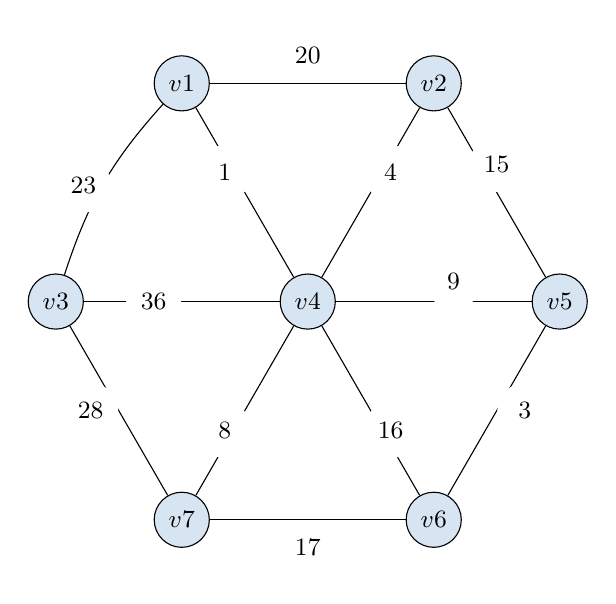
\begin{tikzpicture}[
  scale=1.0,
  every node/.style={circle, draw, fill=nodegray, minimum size=7mm, inner sep=0pt, font=\small},
  w/.style={fill=white, inner sep=1pt, font=\small, draw=none}
]
  \node (v1) at (120:3.2) {$v1$};
  \node (v2) at (60:3.2) {$v2$};
  \node (v5) at (0:3.2) {$v5$};
  \node (v6) at (-60:3.2) {$v6$};
  \node (v7) at (-120:3.2) {$v7$};
  \node (v3) at (180:3.2) {$v3$};
  \node (v4) at (0,0) {$v4$};

  \draw (v1) -- (v2) node[midway, above, w] {20};
  \draw (v1) to[bend right=12] (v3);
  \node[w] at (-2.85,1.48) {23};
  \draw (v1) -- (v4) node[midway, above left, w] {1};
  \draw (v2) -- (v4) node[midway, above right, w] {4};
  \draw (v2) -- (v5) node[midway, above, w] {15};
  \draw (v3) -- (v4) node[midway, left, w] {36};
  \draw (v3) -- (v7) node[midway, left, w] {28};
  \draw (v4) -- (v5) node[midway, above right, w] {9};
  \draw (v4) -- (v6) node[midway, below right, w] {16};
  \draw (v4) -- (v7) node[midway, below left, w] {8};
  \draw (v5) -- (v6) node[midway, right, w] {3};
  \draw (v6) -- (v7) node[midway, below, w] {17};
\end{tikzpicture}
\caption{题目3原图（赋权图$G$）}
\end{figure}

我们先给出图3.34的边信息：
\begin{center}

\begin{tabular}{|c|c|c|}
\hline
编号 & (起点, 终点) & 权值 \\
\hline
1 & $(v1, v2)$ & 20 \\
2 & $(v1, v3)$ & 23 \\
3 & $(v1, v4)$ & 1 \\
4 & $(v2, v4)$ & 4 \\
5 & $(v2, v5)$ & 15 \\
6 & $(v3, v4)$ & 36 \\
7 & $(v3, v7)$ & 28 \\
8 & $(v4, v5)$ & 9 \\
9 & $(v4, v6)$ & 16 \\
10 & $(v4, v7)$ & 8 \\
11 & $(v5, v6)$ & 3 \\
12 & $(v6, v7)$ & 17 \\
\hline
\end{tabular}
\end{center}
我们可以使用 Prim 算法或 Kruskal 算法来求最小生成树，下面分别给出完整过程。

\subsection*{Prim算法}
从 $v1$ 开始，维护已选顶点集合 $S$，每一步选取连接 $S$ 与 $V\setminus S$ 的最小权值边。
\begin{enumerate}
  \item 初始 $S=\{v1\}$，可选边为 $(v1,v2),(v1,v3),(v1,v4)$，选最小边 $(v1,v4)$，权值 $1$。
  \item 此时 $S=\{v1,v4\}$，跨割边中最小的是 $(v4,v2)$，权值 $4$，累计 $1+4=5$。
  \item 此时 $S=\{v1,v2,v4\}$，跨割边中最小的是 $(v4,v7)$，权值 $8$，累计 $13$。
  \item 此时 $S=\{v1,v2,v4,v7\}$，跨割边中最小的是 $(v4,v5)$，权值 $9$，累计 $22$。
  \item 此时 $S=\{v1,v2,v4,v5,v7\}$，跨割边中最小的是 $(v5,v6)$，权值 $3$，累计 $25$。
  \item 此时只剩顶点 $v3$ 未连通，连接到 $v3$ 的候选边为 $(v1,v3),(v7,v3),(v4,v3)$，选最小边 $(v1,v3)$，权值 $23$，累计 $48$。
\end{enumerate}
得到一棵最小生成树：
\[
T=\{(v1,v4),(v2,v4),(v4,v7),(v4,v5),(v5,v6),(v1,v3)\}
\]
总造价为
\[
1+4+8+9+3+23=48.
\]

\subsection*{Kruskal算法}
Kruskal 的思想是：先把所有边按权值从小到大排序，然后依次尝试加入当前边；若加入后不成环，则保留，否则舍弃，直到选出 $n-1=6$ 条边。

将边按权值升序排列为：
\[
\begin{aligned}
&(v1,v4):1,\ (v5,v6):3,\ (v2,v4):4,\ (v4,v7):8,\\
&(v4,v5):9,\ (v2,v5):15,\ (v4,v6):16,\ (v6,v7):17,\\
&(v1,v2):20,\ (v1,v3):23,\ (v3,v7):28,\ (v3,v4):36.
\end{aligned}
\]
下面逐条处理：
\begin{enumerate}
  \item 选 $(v1,v4)$，当前分量：$\{v1,v4\},\{v2\},\{v3\},\{v5\},\{v6\},\{v7\}$。
  \item 选 $(v5,v6)$，当前分量：$\{v1,v4\},\{v2\},\{v3\},\{v5,v6\},\{v7\}$。
  \item 选 $(v2,v4)$，合并后分量：$\{v1,v2,v4\},\{v3\},\{v5,v6\},\{v7\}$。
  \item 选 $(v4,v7)$，合并 后分量：$\{v1,v2,v4,v7\},\{v3\},\{v5,v6\}$。
  \item 选 $(v4,v5)$，合并后分量：$\{v1,v2,v4,v5,v6,v7\},\{v3\}$。
  \item 考察 $(v2,v5)$：两端已在同一分量中，加入会成环，舍弃。
  \item 考察 $(v4,v6)$：两端已在同一分量中，舍弃。
  \item 考察 $(v6,v7)$：两端已在同一分量中，舍弃。
  \item 考察 $(v1,v2)$：两端已在同一分量中，舍弃。
  \item 选 $(v1,v3)$，将 $v3$ 并入主分量，得到单一连通分量，算法结束。
\end{enumerate}
因此 Kruskal 得到的最小生成树边集为
\[
T=\{(v1,v4),(v5,v6),(v2,v4),(v4,v7),(v4,v5),(v1,v3)\},
\]
总造价为
\[
1+3+4+8+9+23=48.
\]

对应的最小生成树示意图如下。

\begin{figure}[h]
\centering
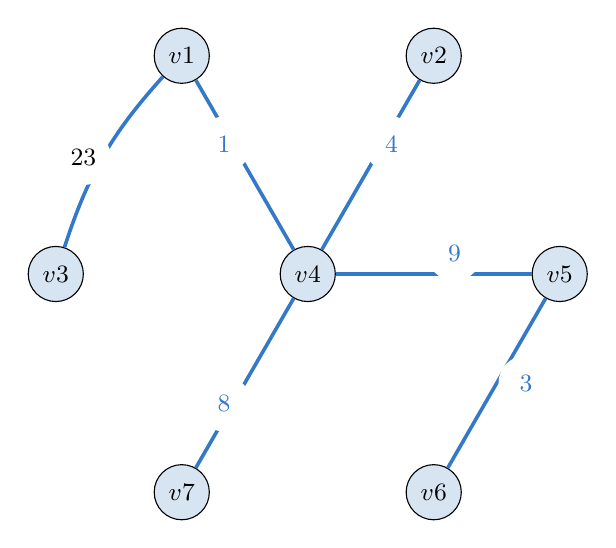
\begin{tikzpicture}[
  scale=1.0,
  every node/.style={circle, draw, fill=nodegray, minimum size=7mm, inner sep=0pt, font=\small},
  mst/.style={line width=1.3pt, color=nodeblue},
  w/.style={fill=white, inner sep=1pt, font=\small, draw=none}
]
  \node (v1) at (120:3.2) {$v1$};
  \node (v2) at (60:3.2) {$v2$};
  \node (v5) at (0:3.2) {$v5$};
  \node (v6) at (-60:3.2) {$v6$};
  \node (v7) at (-120:3.2) {$v7$};
  \node (v3) at (180:3.2) {$v3$};
  \node (v4) at (0,0) {$v4$};

  \draw[mst] (v1) -- (v4) node[midway, above left, w] {1};
  \draw[mst] (v2) -- (v4) node[midway, above right, w] {4};
  \draw[mst] (v4) -- (v7) node[midway, below left, w] {8};
  \draw[mst] (v4) -- (v5) node[midway, above right, w] {9};
  \draw[mst] (v5) -- (v6) node[midway, right, w] {3};
  \draw[mst] (v1) to[bend right=12] (v3);
  \node[w] at (-2.85,1.48) {23};
\end{tikzpicture}
\caption{题目3最小生成树（MST）}
\end{figure}

\end{document}